\chapter{Structurele kwaliteit}
In voorgaande cursussen hebben we geleerd om software 
te analyseren, te ontwerpen en te realiseren.
Daarbij hebben we kennisgemaakt met verschillende
programmeerstijlen in verschillende programmeertalen, 
zoals procedureel programmeren in Python en 
object-georiënteerd programmeren in Java.
Software development is echter méér dan alleen maar code typen!
Wanneer is er sprake van \emph{goede} software?
Hoewel deze vraag door iedereen anders beantwoord zal
worden, zijn er een paar algemene dingen over te zeggen.

We kunnen deze vraag beantwoorden vanuit het perspectief 
van een \emph{gebruiker}. Een gebruiker van de software 
zal zaken als functionaliteit, performance, beveiliging 
en gebruiksvriendelijkheid erg belangrijk vinden. 
Hoe de software er precies van binnen uitziet,
is voor de gebruiker niet rechtstreeks van belang.

Vanuit het perspectief van de \emph{ontwikkelaar}
is dit veel eerder het geval.
Dan kan je bij goede software bijvoorbeeld ook denken 
aan hoe makkelijk het is om de software te begrijpen,
door te ontwikkelen, te veranderen en te testen. Ook het onafhankelijk
kunnen werken aan of testen van programmaonderdelen valt hieronder,
evenals in hoeverre bepaalde onderdelen te vervangen of te hergebruiken zijn.
Bijna niemand vindt het fijn om te werken 
met \emph{spaghetticode} (Figuur~\ref{fig:spaghetticode})!
Deze mate van onderhoudbaarheid (\emph{maintainability}\index{maintainbility}) is over het algemeen
wat men verstaat onder de \emph{structurele kwaliteit} \index{structurele kwaliteit}
van software (\cite{ISO25010} onder 4.2.7).

\begin{figure}[H]
    \centering
    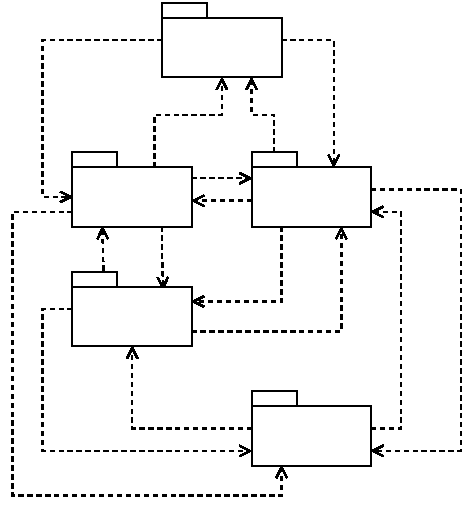
\includegraphics[width=.5\linewidth]{spaghetticode}
    \caption{Als code-onderdelen allemaal afhankelijk van elkaar zijn, 
    is het erg lastig om een onderdeel op zichzelf te wijzigen. 
    Dan spreekt men ook wel van spaghetticode.}
    \label{fig:spaghetticode}
    \index{spaghetticode}
\end{figure}

Natuurlijk kan de interne structuur 
van de software ook gevolgen hebben voor de gebruiker!
Denk bijvoorbeeld aan het tempo waarmee nieuwe features
kunnen worden uitgerold, de prestaties kunnen worden geoptimalizeerd 
of fouten kunnen worden opgespoord en hersteld. 
Het is makkelijker om de software te begrijpen, te veranderen 
of te verbeteren wanneer deze onderhoudbaar is ingericht. 
In projecten met een hoge structurele kwaliteit
zijn concepten duidelijk van elkaar gescheiden en zitten alleen die dingen
bij elkaar in een methode, klasse of package die bij elkaar horen.
Aan de andere kant wordt in dergelijke projecten flexibiliteit behouden
door de software samen te stellen uit verwisselbare onderdelen.
Vaak wordt daarbij gebruik gemaakt van bestaande oplossingen
zoals design patterns, libraries en frameworks, zodat de 
software meer gericht is op het oplossen van het 
daadwerkelijke probleem dan op de details van de uitvoerende technologie.

Het kan ook voorkomen dat een bepaalde nette structuur
minder efficiënt werkt of om een andere reden niet bij de oplossing past. 
In dat soort gevallen kan een ontwikkelaar ervoor kiezen, 
na de precieze impact te meten en de risico's af te wegen, om
op bepaalde plekken in de software voorrang te geven aan de prestaties tegenover 
de structuur. Het verdient aanbeveling om te beginnen met een nette structuur
en dan pas te optimaliseren, omdat binnen een geordende structuur het probleem
makkelijker op te sporen en te verbeteren is. Andersom
is het lastig om bijvoorbeeld performance-gerichte code meer onderhoudbaar te maken.

De beroemde computerwetenschapper 
Donald Knuth wees al decennia geleden op de gevaren van
voortijdige optimalisatie:
\blockquote{
The real problem is that programmers have spent
far too much time worrying about efficiency in the
wrong places and at the wrong times; premature
optimization is the root of all evil (or at least most of it)
in programming.
}{\cite{Knuth1974}, p. 671}

Ook wanneer maar één iemand aan de software werkt, 
is het van belang om aandacht te besteden aan de structuur. 
Het blijkt vaak erg lastig om code van een paar maanden geleden
nog goed te begrijpen! 
Veel developers vragen zich,
in totale verwarring, op enig punt in hun carrière af:
``Waar dacht ik in vredesnaam aan toen ik dit stuk code schreef?!''
Om nog maar te zwijgen over andermans code\ldots

Dit soort verbijstering zal minder plaatsvinden binnen
een georganiseerd project met duidelijke, betekenisvolle
abstracties, overzichtelijk georganiseerd en zonder verrassingen. 
Het is de kunst van een software developer om dit te bereiken!
Vakmannen en -vrouwen willen een doelbewust ontworpen oplossing, gerealiseerd met 
een geschikt gebruik van de programmeertaal volgens best practices, 
principles en patterns gecombineerd met nuttige comments, documentatie en tests.

We hebben nu in grote lijnen een idee gekregen van wat
structurele kwaliteit is. Hoe kunnen we de structuur van software beoordelen?
Hoe kunnen we onze software `netjes' inrichten? Het antwoord is te vinden
in de drie C's van structurele kwaliteit: 
separation of concerns, high cohesion en loose coupling.

\section{Separation of concerns}
\index{seperation of concerns}
Een onderhoudbaar systeem begint bij een systeem dat 
makkelijk te begrijpen is. Het zou mooi zijn als we 
terug kunnen vinden waar wat in ons systeem gebeurt!
Hoe doen we dat in het dagelijks leven?

Neem bijvoorbeeld de inrichting van een lade waar we bestek in doen.
Deze willen we optimaliseren voor het snel kunnen terugvinden
van het juiste bestek: vorken, messen en lepels in allerlei soorten en maten.
Om die reden hebben besteklades vaak een logische indeling, zodat 
het dekken van de tafel (of het opruimen na een afwas) minder tijd en moeite kost.
Het feit dat er een besteklade is waar we het bestek kunnen terugvinden
is natuurlijk ook al handig. Zo hoeven we niet door de hele keuken of eetkamer
te lopen om al het bestek bij elkaar te sprokkelen. 
Sterker nog: we hebben bepaalde voorwerpen (kookgerei, borden, bestek, etcetera) 
in de keuken en eetkamer gezet zodat we niet voor elke maaltijd het hele huis hoeven 
te doorzoeken! Er zijn natuurlijk uitzonderingen, maar we verdelen een huis 
in kamers op basis van de activiteiten die daarin plaatsvinden. 
Als we nog een stap uitzoomen, zie je dat een gemeente vaak ook een doelmatige
indeling heeft op basis van een bestemmingsplan. 
Industrie, woningen, winkelstraten: er zit een logische verdeling in!

Software kunnen we op eenzelfde manier benaderen.
Er zijn verschillende plekken in een softwaresysteem 
waar dingen gebeuren, maar we hoeven niet overal tegelijkertijd te zijn. 
We kunnen terugvinden waar wat precies gebeurt als we 
alle programmaonderdelen voorspelbaar indelen op basis van welke activiteiten
erin gebeuren. Het is dus niet erg om veel doelgerichte 
klassen en packages aan te maken,
mits de indeling en naamgeving bijdraagt 
aan de begrijpelijkheid en vindbaarheid.

Edsger Dijkstra, een van de (Nederlandse) grondleggers van 
softwareontwikkeling als zelfstandig studiegebied, zei het als volgt 
(onze cursivering):
\blockquote{
    Let me try to explain to you, what to my taste is characteristic for all intelligent thinking. 
    It is, that one is willing to study in depth an aspect of one's subject matter 
    \emph{in isolation} for the sake of its own consistency, 
    all the time knowing that one is occupying oneself only with \emph{one of the aspects}. 
    \newline\newline
    (...)
    \newline\newline
    It is what I sometimes have called "the separation of concerns", which, even if not perfectly possible, 
    is yet the only available technique for effective ordering of one's thoughts, 
    that I know of. This is what I mean by "focussing one's attention upon some aspect": 
    it does not mean ignoring the other aspects, it is just doing justice to the fact that 
    from this aspect's point of view, the other is irrelevant. 
    It is being one- and multiple-track minded simultaneously.
}{\cite{Dijkstra1982}, EWD447}

We willen ons systeem zó inrichten dat we verschillende aspecten
in verschillende onderdelen samenbrengen en we ons steeds maar met een
beperkt aantal onderdelen tegelijkertijd hoeven bezig te houden,
wanneer we de code schrijven, testen, verbeteren, 
uitbreiden, verwijderen en vervangen.

\subsection{Modules}
\index{module}
Een groepering van programmaonderdelen noemen we ook wel een \emph{module}.
In klasse-gebaseerde object-georiënteerde talen zoals Java en C\# 
zijn klassen en objecten de meest fundamentele modules. 
Hierin worden toestand en gedrag samengebracht in \emph{fields} en \emph{methods}:
de elementaire delen van een programmastructuur. 
Idealiter ziet een klasse moet op één aspect van functionaliteit 
en zijn de klasse en diens fields en methods voorzien van logische, menselijke namen.

\index{interface}
\emph{Interfaces} zijn andere fundamentele modules. 
Hiermee kan je bepaald gedrag van een subklasse afdwingen.
De publieke methoden van de implementerende klassen 
(diens \emph{application programming interface} of \emph{API}) moeten 
voldoen aan de in de interface opgenomen specificatie.
De methodenamen en parameter- en returntypes moeten overeenkomen met wat 
in de interface wordt afgedwongen.

\index{enumeration}
In veel programmeertalen heb je \emph{enumerations} (enums) 
om een beperkte set aan mogelijkheden aan te geven. Denk bijvoorbeeld aan 
de vier seizoenen van het jaar, de planeten van ons melkwegstelsel 
of de classificatiecodes van films. Met een beetje goede wil kan je 
een boolean zien als een enumeration van true en false.

Ten slotte heb je soms objecten nodig die geen gedrag nodig hebben
maar een groepering van een toestand vertegenwoordigen. 
In C\# kan je dit onderbrengen in een \emph{struct}. 
Sinds Java 16 kan je dit met \emph{records} bereiken.

\subsubsection{Packages}
\index{package}
In het \emph{filesystem} kan je bestanden groeperen door directories aan te maken.
Binnen een directory kan een bestandsnaam geen twee keer voorkomen, 
maar een bestandsnaam kan wel vaker voorkomen als de bestanden in verschillende
directories zitten. Met andere woorden: met directories kan je bestanden
bij elkaar brengen die bij elkaar horen, 
maar ook \emph{naming conflicts} (\emph{collisions}) voorkomen.

Dit is precies hoe Java's \emph{packages} en C\#'s \emph{namespaces} ook worden gebruikt:
om modules te groeperen en botsingen in naamgeving te voorkomen.
Net als directories kennen packages een \emph{recursieve} structuur.
Een package kan namelijk klassen, interfaces, enums en records bevatten, 
maar ook (sub)packages!

Packages zijn erg geschikt om aan te geven in welk algemene deelgebied (subdomein) 
van het softwaresysteem we ons begeven, maar ook om wat voor een soort logica het gaat
of om wat voor een specifieke deelfunctionaliteit het gaat.

\section{Structured design}
\index{structured design}
Het op een logische wijze inrichten van modules 
zorgt er over het algemeen voor dat een systeem makkelijker 
te navigeren is.
Dit zegt echter weinig over hoe je tot \emph{onderhoudbare} modules komt.

Dat was het centrale onderwerp 
van de \emph{structured design}-beweging 
in de jaren zeventig. Het doel was om 
de structurele kwaliteit van software te verbeteren.
Er waren veel problemen met het opdelen 
van software in losstaande onderdelen waar zelfstandig
door verschillende developers of teams aan gewerkt kon worden.
Hoewel het toen niet zozeer ging om object-georiënteerde code,
zijn de toen gevonden problemen, ideeën en oplossingen nog steeds relevant!
\blockquote{
(...) [W]e must be able to make a correction to piece A of the
system without introducing any unanticipated side effects in piece B 
- and, of course, that is precisely the problem that plagues 
many maintenance programmers!
\newline\newline
(...)
\newline\newline
Implementation, maintenance, and modification 
generally will be minimized when each piece of the system
corresponds to exactly one small, well-defined piece of the problem, 
and each relationship between a system's pieces corresponds only 
to a relationship between pieces of the problem.
}{\cite{YourdonConstantine1979}, pp. 17--18}

Bij het creëren van modules willen we erop letten dat 
we zaken groeperen die qua functionaliteit bij elkaar horen.  
Modules mogen alleen met elkaar interacteren voor zover dat 
nodig is voor de uitvoering van een bepaalde taak.
Op die manier verkleinen we de kans dat de wijziging in één onderdeel
automatisch gevolgen heeft voor de werking van een ander onderdeel.
Dit komt overeen met wat wordt verstaan onder \emph{modulariteit}, 
\index{modulariteit}
aldus \cite{ISO25010}: 
"[the] degree to which a system or computer program is composed of 
discrete components such that a change to one component has minimal impact
on other components".

De eigenschappen van modulariteit zijn uitvoerig onderzocht door
Yourdon en Constantine in hun werken over structured design.
Nog altijd analyseren software engineers hun werk aan de hand
van onder andere de termen \emph{cohesion} en \emph{coupling}.

\subsection{Cohesion}
\index{cohesion}
\index{samenhang}
Cohesion (of: \emph{samenhang}) ziet op de binnenkant van een module:
in hoeverre hangen de fields en methods binnen een klasse en de 
klassen binnen een package met elkaar samen?
We mogen immers verwachten dat alle interne elementen van een module 
met een duidelijk doel zijn ontworpen!
\blockquote{
Let us imagine (...) that there is some measure of 
functional (problem-defined) relatedness between pairs
of processing elements. In terms of this measure,
the most effectively modular system is the one for which
the sum of functional relatedness between pairs of elements
not in the same module is minimized; among other things, this
tends to minimize the required amount of intermodular connections
and the amount of intermodular coupling.
\newline\newline
(...)
\newline\newline
What we are considering is the \emph{cohesion} of each module
in isolation -- how tightly bound or related its internal elements
are to one another.
}{\cite{YourdonConstantine1979}, p. 95}

Wanneer een klasse heel veel methoden bevat die elk op een ander stuk
functionaliteit zien of een package allerlei klassen bevat die vrij weinig
met elkaar te maken hebben, spreken we van \emph{low cohesion}. Dit is vaak
een teken om de code te herstructureren. Zie Figuur~\ref{fig:cohesion}.
Meestal willen we dan een klasse opsplitsen
of klassen op een meer samenhangende manier verdelen binnen packages.
We willen ons richten op \emph{high cohesion}: de verantwoordelijkheden van een
klasse of package zien op gelijksoortige onderwerpen of functionaliteiten.
Zo wil je alles dat met security te maken heeft, 
waaronder registreren, inloggen, authentication en authorization,
in een andere module stoppen dan alles dat met het 
opnemen of storten van chips te maken heeft.

\begin{figure}[H]
    \centering
    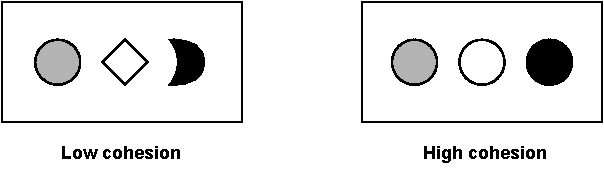
\includegraphics[width=.7\linewidth]{cohesion}
    \caption{Low cohesion versus high cohesion.
    Een samenhangende module brengt verschillende gerelateerde zaken samen 
    en ziet niet op teveel aspecten tegelijkertijd.}
    \label{fig:cohesion}
\end{figure}

Stel je een systeem voor waarin regelmatig een bestand moet worden uitgelezen
en opgeslagen worden van het bestandssysteem. In plaats van dat je op elke plek 
opnieuw op de details van het bestandssysteem in gaat, zou je een toegewijd systeemonderdeel kunnen 
ontwerpen dat enkel verantwoordelijk is voor het lezen en schrijven van bepaalde data.
Op die manier is er één duidelijk punt waarin bestanden worden uitgelezen en weggeschreven.

\subsection{Coupling}
\index{coupling}
\index{koppeling}
Coupling (\emph{koppeling}) ziet op de relaties tussen modules.
In hoeverre is een bepaalde module \emph{afhankelijk} van een andere module?
\blockquote{
The measure that we are seeking is known as \emph{coupling};
it is a measure of the \emph{strength} of interconnection. 
Thus, ``highly coupled'' modules are joined by strong 
interconnections; ``loosely coupled'' modules are joined by
weak interconnections; ``uncoupled'' or ``decoupled'' modules 
have \emph{no} interconnections and are, thus, \emph{independent}
(...). 
\newline\newline
Obviously, what we are striving for is loosely coupled systems
-- that is, systems in which one can study (or debug, or maintain)
any one module without having to know very much about any other
modules in the system.
}{\cite{YourdonConstantine1979}, p. 76}

We willen werken in losgekoppelde systemen. In dat soort systemen
hebben wijzigingen in de ene module slechts een beperkte impact 
op een andere module. Dat komt omdat er spaarzaam wordt omgegaan 
met de afhankelijkheden tussen modules. Er is dan sprake van
\emph{loose coupling}. In de meeste gevallen willen we 
\emph{tight coupling} vermijden. Zie Figuur~\ref{fig:coupling}.

\begin{figure}[H]
    \centering
    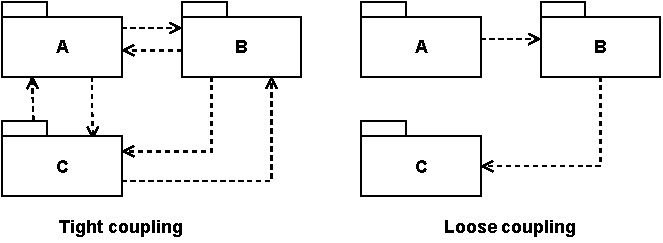
\includegraphics[width=.7\linewidth]{coupling}
    \caption{Tight coupling versus loose coupling.
    In een losgekoppeld systeem wordt er doelbewust omgegaan 
    met afhankelijkheden.}
    \label{fig:coupling}
\end{figure}

\index{afhankelijkheid}
\index{dependency} 
Een andere manier om over coupling na te denken is door te kijken naar hoeveel 
de ene module weet van een andere module. Hierin kan je verschillende gradaties
herkennen: kent de ene module de andere niet, kent deze slechts een publieke methode 
of is deze bekend met alle details die zich binnen de andere module afspelen?
Dat maakt nogal een verschil!

Zie nogmaals het voorbeeld van het bestandssysteem. In plaats van dat we op 
verschillende plekken bezig moeten zijn met de details van opslag, hebben we 
een module gemaakt die verantwoordelijk is voor het uitlezen en wegschrijven 
van bestanden. Gebruikers van die klasse hoeven alleen maar bekend te zijn met de 
diesnten die door die module worden geboden en niet met alle details van bestandsafhandeling.
Op die manier wordt de coupling beperkt.

Een klasse kan op een aantal manieren gekoppeld zijn aan een andere
klasse. Zo kan een object van een bepaalde klasse bijvoorbeeld de publieke methoden
aanroepen van een andere klasse, kan een object zijn opgebouwd uit andere
klassen (\emph{associatie}) of kan er sprake zijn van
overerving (\emph{generalization}) of implementatie (\emph{realisatie}).

Hoewel cohesion (de samenhang binnen een module) 
en coupling (de relatie tussen modules) 
twee verschillende begrippen zijn, is er in de praktijk 
een verband te bespeuren tussen de twee.
\blockquote{
Clearly, cohesion and coupling are interrelated. The greater
the cohesion of individual modules in the system, the lower
the coupling between modules will be. In actual practice,
these two measures are correlated; that is, on the average,
as one increases, the other decreases; but the correlation is 
not perfect.
}{\cite{YourdonConstantine1979}, p. 96}

Over het algemeen kunnen we dus zeggen dat de mate van koppeling
tussen modules kleiner is wanneer modules meer interne samenhang vertonen.
Modules hoeven dan immers minder informatie met elkaar te delen.

\section{Samenvatting}
In dit hoofdstuk hebben we onderzocht wat we kunnen verstaan onder
structurele kwaliteit en hoe we dit over het algemeen kunnen bereiken.

\begin{defbox}{Structurele kwaliteit}
    Structurele kwaliteit ziet vooral op de onderhoudbaarheid
    van een softwareproject.
    \newline\newline
    Een softwareproject heeft in algemene zin 
    een goede structuur als deze is opgedeeld in kleine,
    opzichzelf staande modules die intern veel samenhang 
    en met elkaar beperkt koppeling vertonen.
    \newline\newline
    Met andere woorden, we willen modulariteit dankzij:
    \begin{enumerate}
        \item Separation of concerns
        \item High cohesion
        \item Loose coupling
    \end{enumerate}
\end{defbox}


